%%%%%%%%%%%%%%%%%%%%%%%%%%%%%%%%%%%%%%%%%%%%%%%%%%%%%%%%%%%%%%%%%%%%%%%%%%%%%%%%%%%%%%%%%%%%%%%%%%%%%
% DOCUMENT CLASS
%%%%%%%%%%%%%%%%%%%%%%%%%%%%%%%%%%%%%%%%%%%%%%%%%%%%%%%%%%%%%%%%%%%%%%%%%%%%%%%%%%%%%%%%%%%%%%%%%%%%%%

%\documentclass[journal=jacsat,manuscript=article]{achemso}

% Single-spaced, two-column with PRL look and style (easy on the eyes)
\documentclass[aps,pre,twocolumn,nofootinbib,superscriptaddress,linenumbers]{revtex4-1}


% Double-spaced, one-column style (for submission/review/editing)
%\documentclass[aps,preprint,prl,superscriptaddress,showpacs]{revtex4}

%%%%%%%%%%%%%%%%%%%%%%%%%%%%%%%%%%%%%%%%%%%%%%%%%%%%%%%%%%%%%%%%%%%%%%%%%%%%%%%%%%%%%%%%%%%%%%%%%%%%%%
% PREAMBLE
%%%%%%%%%%%%%%%%%%%%%%%%%%%%%%%%%%%%%%%%%%%%%%%%%%%%%%%%%%%%%%%%%%%%%%%%%%%%%%%%%%%%%%%%%%%%%%%%%%%%%%

% FONT
\usepackage{palatino}

\usepackage{amsmath}
\usepackage{amssymb}
\usepackage{graphicx}
\usepackage{dcolumn}
\usepackage{boxedminipage}
\usepackage{verbatim}
\usepackage{booktabs}

\usepackage[colorlinks=true,citecolor=blue,linkcolor=blue]{hyperref}

% The figures are in a figures/ subdirectory.
\graphicspath{{../figures/}}

%\bibliographystyle{apsrevlong}
\bibliographystyle{apsrev}

% italicized boldface for math (e.g. vectors)
\newcommand{\bfv}[1]{{\mbox{\boldmath{$#1$}}}}
% non-italicized boldface for math (e.g. matrices)
\newcommand{\bfm}[1]{{\bf #1}}          

%\newcommand{\bfm}[1]{{\mbox{\boldmath{$#1$}}}}
%\newcommand{\bfm}[1]{{\bf #1}}
\newcommand{\expect}[1]{\left \langle #1 \right \rangle}                % <.> for denoting expectations over realizations of an experiment or thermal averages
\newcommand{\dhdl}{\frac{dH}{d\lambda}}
% vectors
\newcommand{\var}[1]{{\mathrm var}{(#1)}}
\newcommand{\x}{\bfv{x}}
\newcommand{\y}{\bfv{y}}
\newcommand{\f}{\bfv{f}}

\newcommand{\bfc}{\bfm{c}}
\newcommand{\hatf}{\hat{f}}

\newcommand{\bTheta}{\bfm{\Theta}}
\newcommand{\btheta}{\bfm{\theta}}
\newcommand{\bhatf}{\bfm{\hat{f}}}
\newcommand{\Cov}[1] {\mathrm{cov}\left( #1 \right)}
\newcommand{\Ept}[1] {{\mathrm E}\left[ #1 \right]}
\newcommand{\Eptk}[2] {{\mathrm E}_{#1}\left[ #2\right]}
\newcommand{\T}{\mathrm{T}}                                % T used in matrix transpose

%%%%%%%%%%%%%%%%%%%%%%%%%%%%%%%%%%%%%%%%%%%%%%%%%%%%%%%%%%%%%%%%%%%%%%%%%%%%%%%%
% DOCUMENT
%%%%%%%%%%%%%%%%%%%%%%%%%%%%%%%%%%%%%%%%%%%%%%%%%%%%%%%%%%%%%%%%%%%%%%%%%%%%%%%%

\begin{document}

%%%%%%%%%%%%%%%%%%%%%%%%%%%%%%%%%%%%%%%%%%%%%%%%%%%%%%%%%%%%%%%%%%%%%%%%%%%%%%%%
% TITLE AND AUTHORS
%%%%%%%%%%%%%%%%%%%%%%%%%%%%%%%%%%%%%%%%%%%%%%%%%%%%%%%%%%%%%%%%%%%%%%%%%%%%%%%%

\title{Benchmarking Simulations against the ThermoML Database:\\
Neat Liquid Densities and Static Dielectrics}

\author{Kyle A. Beauchamp$^+$}
\email{kyle.beauchamp@choderalab.org}
\affiliation{Computational Biology Program, Memorial Sloan Kettering Cancer Center, New York, NY}

\author{Julie M. Behr$^+$}
\email{julie.behr@choderalab.org}
\affiliation{Tri-Institutional Program in Computational Biology and Medicine, Weill Cornell Medical College, New York, NY}

\author{Patrick B. Grinaway }
\email{patrick.grinaway@choderalab.org}
\affiliation{Graduate Program in Physiology, Biophysics, and Systems Biology, Weill Cornell Medical College, New York, NY}

\author{Arien S. Rustenburg}
\email{bas.rustenburg@choderalab.org}
\affiliation{Graduate Program in Physiology, Biophysics, and Systems Biology, Weill Cornell Medical College, New York, NY}
 
 \author{Kenneth Kroenlein}
 \email{kenneth.kroenlein@nist.gov}
 \affiliation{NIST Thermodynamics Research Center, Boulder, CO}
 
 \author{John D. Chodera}
 \thanks{Corresponding author}
 \email{john.chodera@choderalab.org}
 \affiliation{Computational Biology Program, Memorial Sloan Kettering Cancer Center, New York, NY}

\date{\today}

%%%%%%%%%%%%%%%%%%%%%%%%%%%%%%%%%%%%%%%%%%%%%%%%%%%%%%%%%%%%%%%%%%%%%%%%%%%%%%%%
% ABSTRACT
%%%%%%%%%%%%%%%%%%%%%%%%%%%%%%%%%%%%%%%%%%%%%%%%%%%%%%%%%%%%%%%%%%%%%%%%%%%%%%%%

%\section{Abstract}
\begin{abstract}

Useful atomistic simulations in the condensed phase require accurate depictions of solvent.  
While accurate experimental measurements of fundamental physical properties offer a straightforward approach for evaluating forcefield quality, the bulk of this information has been tied up in non-machine-readable formats that pose many risks to the automated evaluation of forcefield accuracy.
Here we examine the feasibility of benchmarking atomistic forcefields against the NIST ThermoML database of physicochemical measurements, which aggregates thousands off experimental measurements in a portable machine-readable self-annotating format. 
We present a detailed benchmark of the generalized Amber small molecule forcefield (GAFF) using the AM1-BCC charge model against measurements (specifically liquid densities and static dielectric constants at ambient pressure) extracted from ThermoML, and discuss the extent of available data for neat liquids.  
{\color{red} We show that empirical polarizability models correct systematic biases inherent in predicting dielectric constants with fixed-charged forcefields.  [JDC: Will need to be convinced!]}

\emph{Keywords: molecular mechanics forcefields; forcefield parameterization; forcefield accuracy; forcefield validation; mass density; static dielectric constant}

\end{abstract}

\maketitle

%%%%%%%%%%%%%%%%%%%%%%%%%%%%%%%%%%%%%%%%%%%%%%%%%%%%%%%%%%%%%%%%%%%%%%%%%%%%%%%%
% INTRODUCTION
%%%%%%%%%%%%%%%%%%%%%%%%%%%%%%%%%%%%%%%%%%%%%%%%%%%%%%%%%%%%%%%%%%%%%%%%%%%%%%%%

\section{Introduction}

Recent advances in hardware and molecular dynamics software have provided routine access to atomistic simulations at the 100 ns timescale and beyond. 
Leveraging these advances in combination with GPU clusters, distributed computing, or custom hardware has brought the microsecond and milliseconds within reach.  
These dramatic advances in sampling, however, have revealed forcefields as a critical barrier for truly predictive simulation.  

Protein and water forcefields have been the subject of numerous benchmarks~\cite{} and enhancements~\cite{}, with key outcomes including the ability to fold fast-folding proteins, improved fidelity of water thermodynamic properties, and improved prediction of NMR observables.  
Although small molecule forcefields have also been the subject of benchmarks~\cite{} and improvements~\cite{}, such work has focused on small perturbations to specific functional groups.  
For example, a recent study found that modified hydroxyl nonbonded parameters led to improved prediction of static dielectrics and hydration free energies.  
%Other studies have found XYZ.  
There are also outstanding questions of generalizability of parameters.  
Will changes to a specific chemical moiety be compatible with seemingly unrelated improvements?  
Addressing these questions requires agreement on shared benchmarks that can be easily replicated with proposed forcefield enhancements.

A key barrier in forcefield development is that many experimental datasets are heterogeneous, paywalled, and unavailable in machine-readable formats (although notable counterexamples exist, e.g. RSCB~\cite{}, FreeSolv~\cite{freesolv} and BMRB~\cite{}).  
While this inconvenience is relatively minor for benchmarking a single target (e.g. water), it becomes prohibitive for studies spanning chemical space.  
To ameliorate problems of data archival, the NIST Thermodynamics Research Center has developed a IUPAC standard XML-based format---ThermoML \cite{}---for storing physicochemical measurements, uncertainties, and metadata.
 Experimental researchers publishing measurements in several journals (J.~Chem.~Eng.~Data, J.~Chem.~Therm., Fluid Phase Equil., Therm.~Acta, and Int.~J.~Therm.) are now guided through a data archival process that involves sanity checks and eventual archival at the TRC (\url{http://trc.nist.gov/ThermoML.html}).  

Here we examine the ThermoML archive as a potential source for neat liquid density and static dielectric measurements, with the goal of developing a standard benchmark for validating these properties in fixed-charge forcefields of drug-like molecules.  
These two observables provide sensitive tests of forcefield accuracy that are nonetheless straightforward to calculate.  
Using the ThermoML data, we evaluate the generalized Amber small molecule forcefield (GAFF)~\cite{gaff} with the AM1-BCC charge model~\cite{am1bcc1,am1bcc2} and identify systematic biases that might be improved upon.

%%%%%%%%%%%%%%%%%%%%%%%%%%%%%%%%%%%%%%%%%%%%%%%%%%%%%%%%%%%%%%%%%%%%%%%%%%%%%%%%
% RESULTS
%%%%%%%%%%%%%%%%%%%%%%%%%%%%%%%%%%%%%%%%%%%%%%%%%%%%%%%%%%%%%%%%%%%%%%%%%%%%%%%%

\section{Results}

\subsection{Neat Liquid Measurements in ThermoML}

We performed a number of queries to summarize the ThermoML content relevant for benchmarking organic molecule forcefields.  
Our aim is to explore neat liquid data with functional groups relevant to drug-like molecules.  
We therefore applied the following sequence of filters: has either density or static dielectric measurements, contains a single component, contains only druglike elements (H, N, C, O, S, P, F, Cl, Br), has low heavy atom count $(\le 10)$, has ambient temperature [K] $(270 \le T \le 330)$, has ambient pressure [kPA] $(100 \le P \le 102)$, and has density greater than 300 kg $m^{-3}$ (a proxy for liquid state).  
After applying these filters, we also round all pressures within this range to exactly one atmosphere.  We also round temperatures to one decimal place.  
These approximations are motived by common data entry errors; for example, an experiment performed at water's freezing point at ambient pressure might be entered as either 101.325 kPA or 100 kPA, with a temperature of either 273 K or 273.15 K.  
After the application of these filters (Table \ref{table:ThermoMLSummary}), we are left with 245 conditions for which both density and dielectric data are available.  
The functional groups present are summarized in Table \ref{table:ThermoMLSummary}.  

%%%%%%%%%%%%%%%%%%%%%%%%%%%%%%%%%%%%%%%%%%%%%%%%%%%%%%%%%%%%%%%%%%%%%%%%%%%%%%%%
% TABLE: DENSITY AND STATIC DIELECTRIC
%%%%%%%%%%%%%%%%%%%%%%%%%%%%%%%%%%%%%%%%%%%%%%%%%%%%%%%%%%%%%%%%%%%%%%%%%%%%%%%%

\begin{table}
\begin{tabular}{lrr}
\toprule
Filter &  Mass Density &  Static Dielectric \\ 
\midrule
0.  Single Component   &               130074 &                                     1649 \\
1.  Druglike Elements  &               120410 &                                     1649 \\
2.  Heavy Atoms        &                67897 &                                     1567 \\
3.  Temperature        &                36827 &                                      962 \\
4.  Pressure           &                13598 &                                      461 \\
5.  Liquid state       &                13573 &                                      461 \\
6.  Aggregate T, P     &                 3573 &                                      432 \\
7.  Density+Dielectric &                  245 &                                      245 \\
\bottomrule
\end{tabular}
\caption{{\bf Number of ThermoML measurements matching sequentially applied filters.}}
\label{table:ThermoMLSummary}
\end{table}

\begin{table}
\begin{tabular}{lr}
\toprule
Functional Group &    Counts \\
\midrule
1,2-aminoalcohol                                    &   4 \\
1,2-diol                                            &   3 \\
alkene                                              &   3 \\
aromatic compound                                   &   1 \\
carbonic acid diester                               &   2 \\
carboxylic acid ester                               &   4 \\
dialkyl ether                                       &   7 \\
heterocyclic compound                               &   3 \\
ketone                                              &   2 \\
lactone                                             &   1 \\
primary alcohol                                     &  19 \\
primary aliphatic amine (alkylamine)                &   2 \\
primary amine                                       &   2 \\
secondary alcohol                                   &   4 \\
secondary aliphatic amine (dialkylamine)            &   2 \\
secondary aliphatic/aromatic amine (alkylarylamine) &   1 \\
secondary amine                                     &   3 \\
sulfone                                             &   1 \\
sulfoxide                                           &   1 \\
tertiary aliphatic amine (trialkylamine)            &   3 \\
tertiary amine                                      &   3 \\
\bottomrule
\end{tabular}
\caption{Functional group counts present in the dataset.  
The number of unique compounds is 44.  
Functional group classification was performed using checkmol version 0.5 \cite{haider2010functionality}.}
\label{table:FunctionalGroups}
\end{table}

%%%%%%%%%%%%%%%%%%%%%%%%%%%%%%%%%%%%%%%%%%%%%%%%%%%%%%%%%%%%%%%%%%%%%%%%%%%%%%%%
% DENSITY
%%%%%%%%%%%%%%%%%%%%%%%%%%%%%%%%%%%%%%%%%%%%%%%%%%%%%%%%%%%%%%%%%%%%%%%%%%%%%%%%

\subsection{Benchmarking GAFF against ThermoML: Mass Density}

Mass density has been widely used as a critical ingredient for parameterizing and testing forcefields, particularly the Lennard Jones parameters \cite{jorgensen1983comparison, jorgensen1984optimized}.  
We therefore used the present ThermoML compilation as a benchmark of the GAFF AM1-BCC forcefield (Fig. \ref{figure:Density}).  
Overall, the densities show reasonable accuracy (R2 + errobars), consistent with previous studies \cite{caleman2011force} reporting agreement of XYZ on a different benchmark set.  

%%%%%%%%%%%%%%%%%%%%%%%%%%%%%%%%%%%%%%%%%%%%%%%%%%%%%%%%%%%%%%%%%%%%%%%%%%%%%%%%
% FIGURE: DENSITY COMPARISON
%%%%%%%%%%%%%%%%%%%%%%%%%%%%%%%%%%%%%%%%%%%%%%%%%%%%%%%%%%%%%%%%%%%%%%%%%%%%%%%%

\begin{figure}
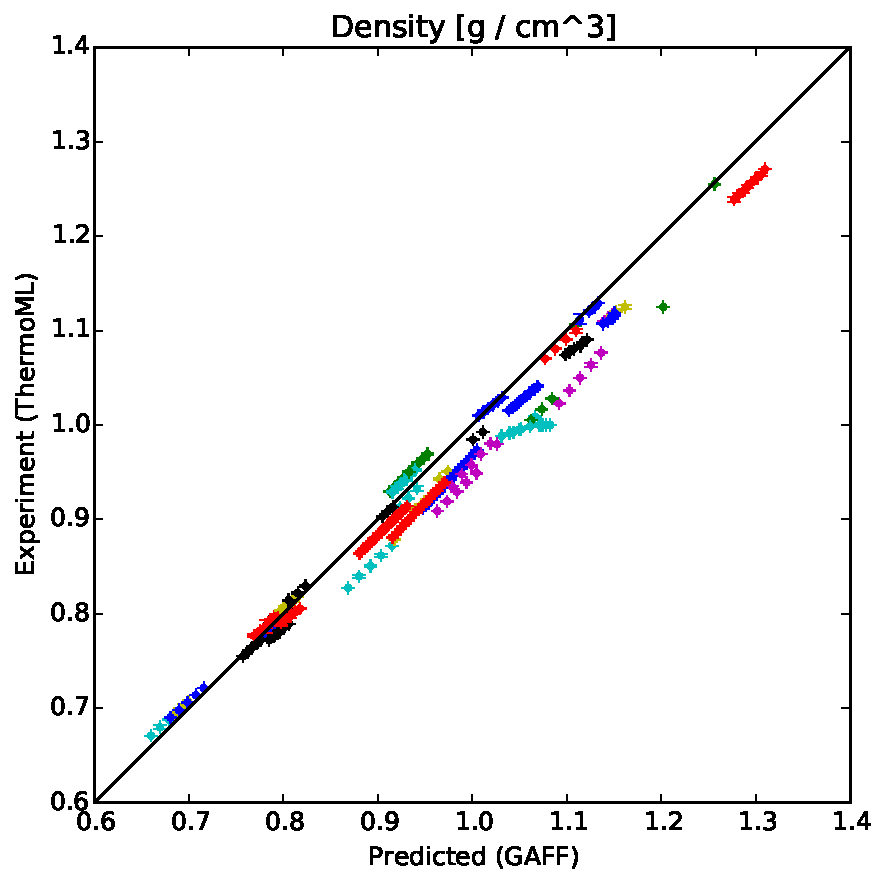
\includegraphics[width=\columnwidth]{./figures/densities_thermoml.pdf}
\caption{{\bf Comparison of liquid densities between experiment and simulation.}
Liquid density measurements at ambient (1 atm) pressure extracted from ThermoML are compared against simulated densities at ambient pressure using the GAFF/AM1-BCC small molecule fixed-charge forcefield.
Color groupings represent identical chemical formulas.  
{\color{red}[JDC: Chemical \emph{species}?]}
Simulation error bars represent one standard error of the mean, with the number of effective (uncorrelated) samples estimated using pymbar.  
Experimental error bars indicate the standard deviation between independently reported measurements, when available, or author-reported standard deviations in ThermoML entries; for some measurements, neither uncertainty estimate is available.  
See {\bf Section~\ref{section:experimental-error}} for further discussion of error.
}
\label{figure:Density}
\end{figure}

%%%%%%%%%%%%%%%%%%%%%%%%%%%%%%%%%%%%%%%%%%%%%%%%%%%%%%%%%%%%%%%%%%%%%%%%%%%%%%%%
% DIELECTRIC
%%%%%%%%%%%%%%%%%%%%%%%%%%%%%%%%%%%%%%%%%%%%%%%%%%%%%%%%%%%%%%%%%%%%%%%%%%%%%%%%

\subsection{Benchmarking GAFF against ThermoML: Static Dielectric}

As a measure of the electronic medium, the static dielectric constant of neat liquids provides a critical benchmark that is somewhat orthogonal to density and thermodynamic quantities.  
We therefore compare simulations against the measurements in our ThermoML compilation.  
Overall, we find the dielectric constants to be qualitatively reasonable, but with clear deviations from experiment.  
In particular, GAFF AM1-BCC systematically underestimates the dielectric constants for nonpolar organics, with GAFF predictions of $\epsilon \approx 1.0 \pm 0.05$ being substantially smaller than the measured $\epsilon \approx 2$.  
Because this deviation likely stems from the lack of electronic polarization, we added a simple empirical correction for polarization \cite{bosque2002polarizabilities}, which leads to better agreement with experiment.  
A similar polarization correction was used in the development of the TIP4P-EW water model \cite{horn2004}; however, the need is much greater for the nonpolar organics, as the missing polarizability is the dominant contribution to the static dielectric constant.  
In the case of water, the Sales polarizability model predicts a dielectric correction of 0.52, while 0.79 was used for the TIP4P-EW model.  
For comparison, we also applied the same empirical correction to the VirtualChemistry dataset \cite{caleman2011force, van2012gromacs} and saw similarly improved agreement with experiment for both the GAFF and OPLS forcefields (Fig. \ref{figure:VirtualChemistry}).

%%%%%%%%%%%%%%%%%%%%%%%%%%%%%%%%%%%%%%%%%%%%%%%%%%%%%%%%%%%%%%%%%%%%%%%%%%%%%%%%
% FIGURE: DIELECTRIC COMPARISON
%%%%%%%%%%%%%%%%%%%%%%%%%%%%%%%%%%%%%%%%%%%%%%%%%%%%%%%%%%%%%%%%%%%%%%%%%%%%%%%%

\begin{figure}
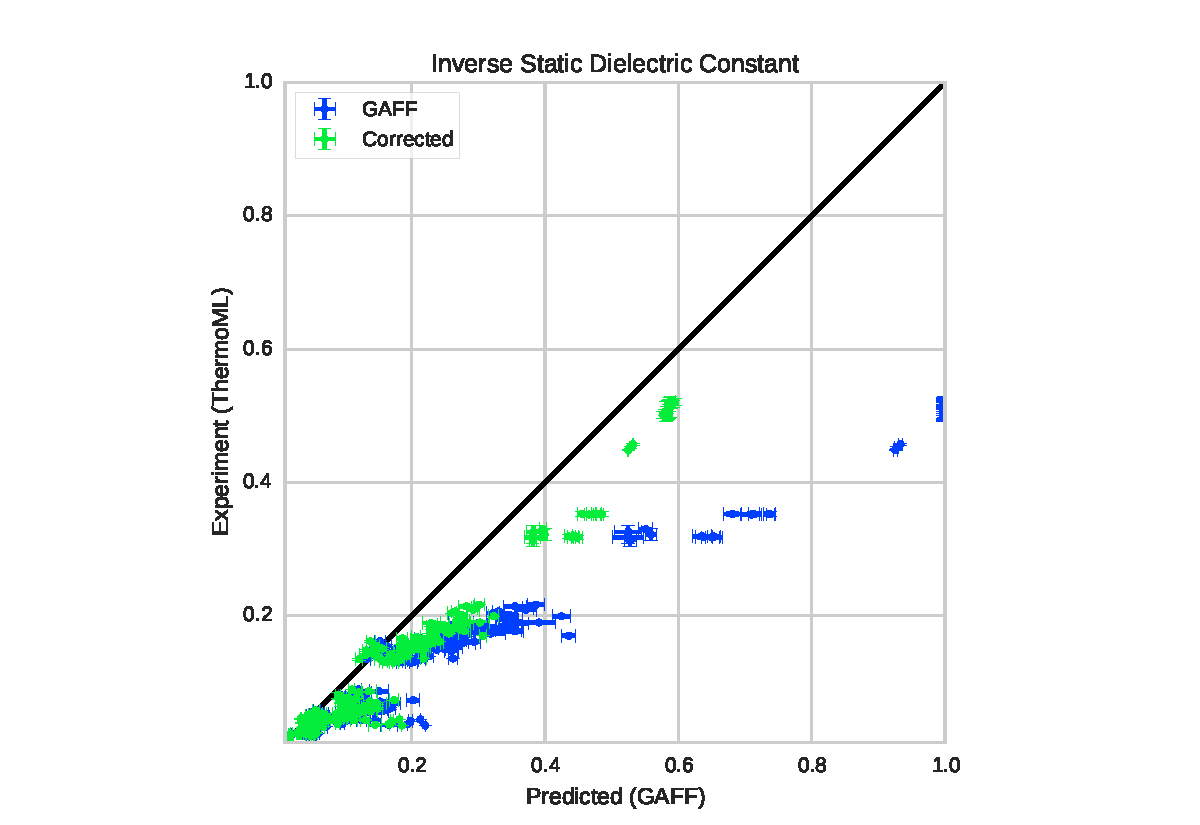
\includegraphics[width=\columnwidth]{./figures/dielectrics_thermoml.pdf}

\caption{{\bf Measured (ThermoML) versus predicted (GAFF) inverse static dielectrics (a).}
Color groupings represent identical chemical formulas.  Simulation error bars represent one standard error of the mean estimated via block averaging with block sizes of 200 ps \cite{flyvbjerg1989error}.  
Experimental error bars indicate the larger of standard deviation between independently reported measurements and the authors reported standard deviations; for some measurements, neither uncertainty estimate is available.  
See section S2 for further discussion of error.  
The inverse dielectric $\frac{1}{\epsilon}$ is plotted instead of $\epsilon$ because $\frac{1}{\epsilon}$ is directly proportional to energy in continuum dielectric models: e.g. $U(r) = \frac{1}{4 \pi \epsilon} \frac{q_1 q_2}{r} \propto \frac{1}{\epsilon}$.
}
\label{figure:Dielectric}
\end{figure}

%%%%%%%%%%%%%%%%%%%%%%%%%%%%%%%%%%%%%%%%%%%%%%%%%%%%%%%%%%%%%%%%%%%%%%%%%%%%%%%%
% DISCUSSION
%%%%%%%%%%%%%%%%%%%%%%%%%%%%%%%%%%%%%%%%%%%%%%%%%%%%%%%%%%%%%%%%%%%%%%%%%%%%%%%%

\section{Discussion}

\subsection{Examining discrepancies by functional group}

%%%%%%%%%%%%%%%%%%%%%%%%%%%%%%%%%%%%%%%%%%%%%%%%%%%%%%%%%%%%%%%%%%%%%%%%%%%%%%%%
% FIGURE: ACCURACY BY FUNCTIONAL GROUP
%%%%%%%%%%%%%%%%%%%%%%%%%%%%%%%%%%%%%%%%%%%%%%%%%%%%%%%%%%%%%%%%%%%%%%%%%%%%%%%%

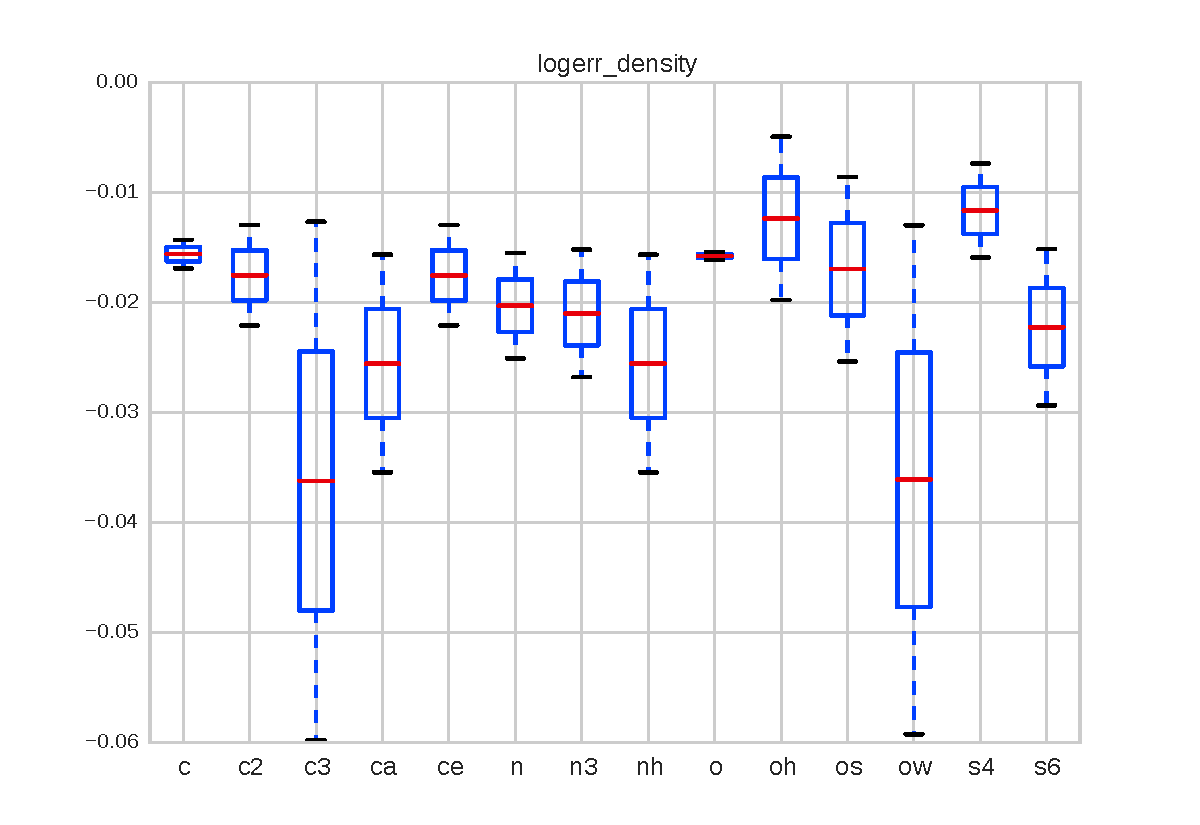
\includegraphics[width=\columnwidth]{./figures/functional_group_logerr_density.pdf}

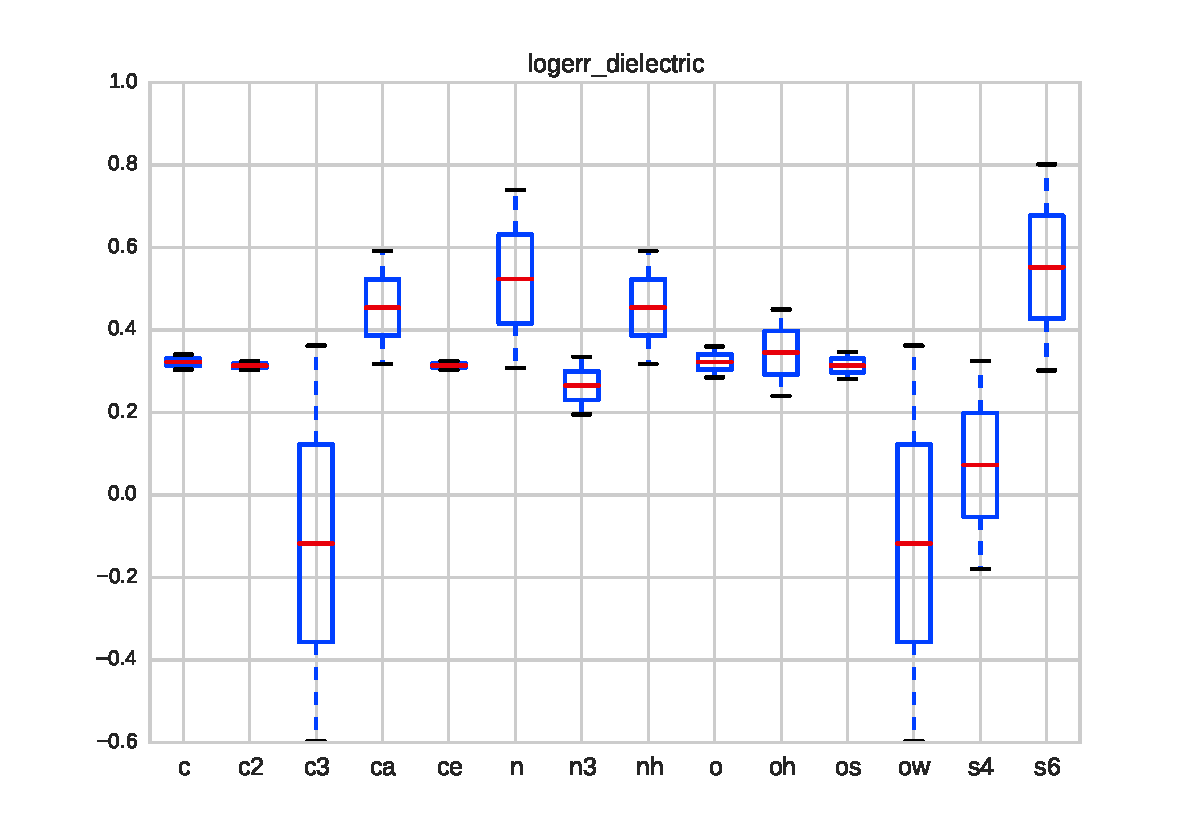
\includegraphics[width=\columnwidth]{./figures/functional_group_logerr_dielectric.pdf}

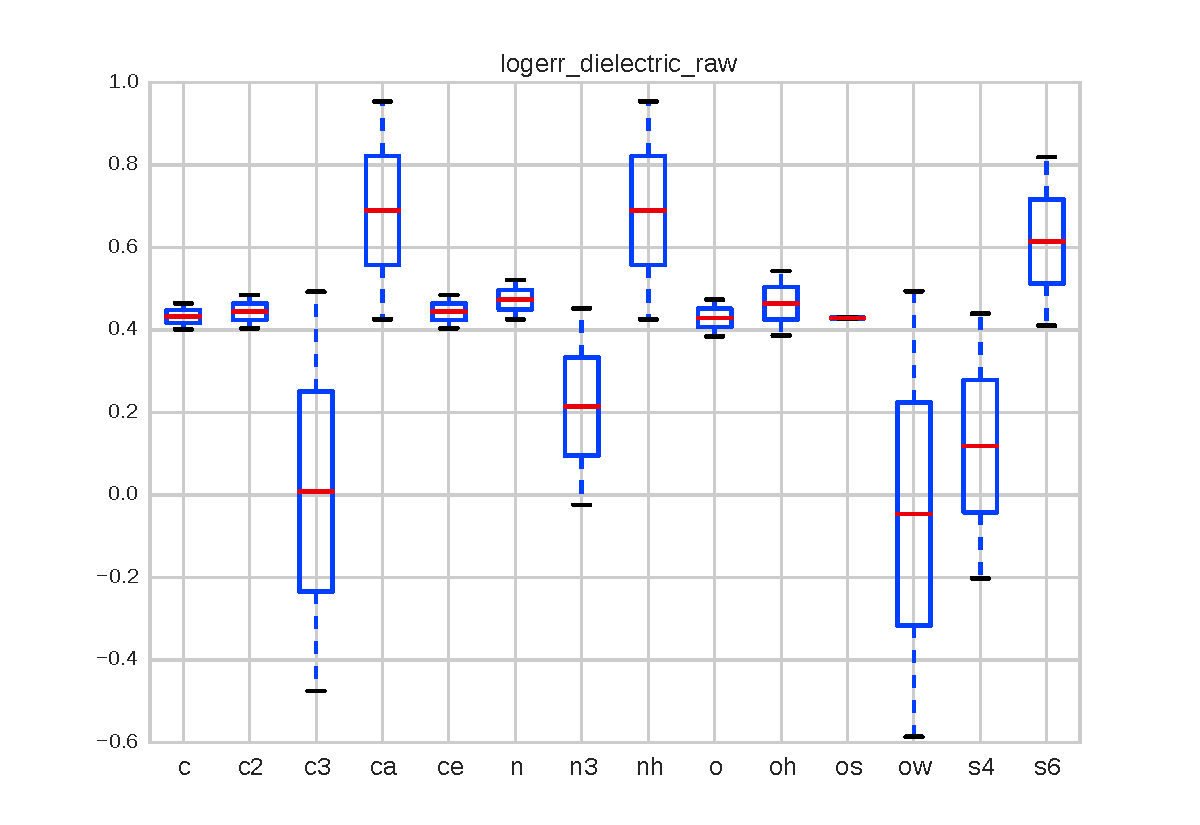
\includegraphics[width=\columnwidth]{./figures/functional_group_logerr_dielectric_raw.pdf}

%%%%%%%%%%%%%%%%%%%%%%%%%%%%%%%%%%%%%%%%%%%%%%%%%%%%%%%%%%%%%%%%%%%%%%%%%%%%%%%%
% FITTING FORCEFIELDS TO DIELECTRIC CONSTANTS
%%%%%%%%%%%%%%%%%%%%%%%%%%%%%%%%%%%%%%%%%%%%%%%%%%%%%%%%%%%%%%%%%%%%%%%%%%%%%%%%

\subsection{Fitting Forcefields to Dielectric Constants}

Recent forcefield development has seen a resurgence of papers fitting dielectric constants as primary data \cite{wang2014building, fennell2014fixed}.  
However, a number of authors have pointed out potential challenges in constructing self-consistent fixed-charge force fields \cite{fennell2012simple, leontyev2014polarizable}.  
Interestingly, a recent work by Dill \cite{fennell2012simple} pointed out that, for $\mathrm{CCl_4}$, reasonable choices of point charges are incapable of recapitulating the observed dielectric of $\epsilon = 2.2$, instead producing dielectric constants in the range of $1.0 \le \epsilon \le 1.05$.  
Suppose, for example, that one attempts to directly fit the static dielectric constants of $\mathrm{CCl_4}$, $\mathrm{CHCl_3}$, $\mathrm{CH_2Cl_2}$, $\mathrm{CH_3Cl_1}$, $\mathrm{CH_4}$.  
In moving from the tetrahedrally-symmetric $\mathrm{CCl_4}$ to $\mathrm{CHCl_3}$, it suddenly becomes possible to achieve the observed dielectric constant of 4.8.  
However, the model for $\mathrm{CHCl_3}$ uses fixed point charges to account for \emph{both} the net dipole moment and the (electronic) polarizability, whereas the $\mathrm{CCl_4}$ model contains no treatment of polarizability.  
We hypothesize that this inconsistency in parameterization may lead to strange mismatches, where symmetric molecules (e.g. benzene, $\mathrm{CCl_4}$) have qualitatively different properties than closely related asymmetric molecules (e.g. toluene, $\mathrm{CHCl_3}$).  
As a first-order fix, we suggest using empirical polarization corrections before directly comparing measured static dielectric constants to fixed-charge models---particularly when examining low-dielectric solvents.  
Separating the contributions of fixed charges and polarization may also lead to the development of improved models of electrostatics that account for the missing polarization physics; some such models have been proposed recently \cite{leontyev2014polarizable}.


\subsection{ThermoML as a Data Source}

The present work has focused on the neat liquid density and dielectric measurements present in ThermoML \cite{frenkel2006xml, frenkel2003thermoml, chirico2003thermoml} as a target for molecular dynamics forcefield validation.  
While densities and dielectric constants have been widely used in forcefield work, several aspects of ThermoML make it a unique resource for the forcefield community.  
First, the aggregation, support, and dissemination of ThermoML is supported by NIST, whose mission makes these tasks a long-term priority.  
Second, ThermoML is actively growing, through partnerships with journals such as J. Chem. Thermo--new experimental measurements published in these journals are critically examined by the TRC and included in the archive.  
Finally, the files in ThermoML are machine readable via a formal XML schema, allowing facile access to thousands of measurements.  
In the future, we hope to examine additional measurement classes, including both mixture and two-phase data.

%%%%%%%%%%%%%%%%%%%%%%%%%%%%%%%%%%%%%%%%%%%%%%%%%%%%%%%%%%%%%%%%%%%%%%%%%%%%%%%%
% METHODS
%%%%%%%%%%%%%%%%%%%%%%%%%%%%%%%%%%%%%%%%%%%%%%%%%%%%%%%%%%%%%%%%%%%%%%%%%%%%%%%%

\section{Methods}

\subsection{ThermoML Processing}

ThermoML XML files were obtained from the the NIST TRC.  To explore their content, we created a python (version 2.7.9) tool (ThermoPyl: \url{https://github.com/choderalab/ThermoPyL}) that munges the XML content into a spreadsheet-like format accessible via the  Pandas (version 0.15.2) library.  
First, we obtained the XML schema (\url{http://media.iupac.org/namespaces/ThermoML/ThermoML.xsd}) defining the layout of the data.  
This schema was converted into a Python object via PyXB 1.2.4 (\url{http://pyxb.sourceforge.net/}).  
Finally, this schema and Pandas was used to extract the data and apply the data filters described above.  

\subsection{Simulation}
Boxes of 1000 molecules were constructed using PackMol \cite{martinez2009packmol}. 
AM1-BCC~\cite{am1bcc1,am1bcc2} charges were generated using OpenEye Toolkit 2014-6-6 \cite{openeye}, using the {\tt oequacpac.OEAssignPartialCharges} module with the {\tt OECharges\_AM1BCCSym}.  
The selected conformer was then processed using antechamber in AmberTools~14~\cite{amber14}.  
The resulting AMBER files were converted to OpenMM~\cite{eastman2012openmm} ffxml forcefield XML files.  
Simulation code used libraries gaff2xml~0.6, TrustButVerify~0.1, OpenMM~6.2~\cite{eastman2012openmm}, and MDTraj~1.2~\cite{mcgibbon2014mdtraj}.  
{\color{red}[TODO: Provide a script to install all of these versions via {\tt conda}.]}

Molecular dynamics simulations were performed using OpenMM~6.2~\cite{eastman2012openmm} using a Langevin integrator (with collision rate 1 ps$^{-1}$) and a 1~fs timestep; interestingly, we found that a 2~fs timestep led to insufficient accuracy in equilibrium densities (Table~\ref{table:TimestepDependence}).  
{\color{red}[JDC: Cite Langevin integrator used in OpenMM.]}
Pressure coupling at 1 atmosphere was achieved with a Monte Carlo barostat utilizing molecular scaling and automated step size adjustment during equilibration, applied every 25 steps.  
Particle mesh Ewald~\cite{Darden1993} was used with a long-range cutoff of 0.95~nm and an long-range isotropic dispersion correction.  
{\color{red}[JDC: Can we report the automatically-selected PME parameters?]}
Simulations were continued until density standard errors were less than $2 \times 10^{-4}$ g / mL, as estimated using the equilibration detection module in pymbar 2.1~\cite{shirts2008statistically}.  
Trajectory analysis was performed using OpenMM~\cite{eastman2012openmm} and MDTraj~\cite{mcgibbon2014mdtraj}.  
Density data was output every 250~fs, while trajectory data was stored every 10~ps.  

%%%%%%%%%%%%%%%%%%%%%%%%%%%%%%%%%%%%%%%%%%%%%%%%%%%%%%%%%%%%%%%%%%%%%%%%%%%%%%%%
% CONCLUSIONS
%%%%%%%%%%%%%%%%%%%%%%%%%%%%%%%%%%%%%%%%%%%%%%%%%%%%%%%%%%%%%%%%%%%%%%%%%%%%%%%%

\section{Conclusions}

\begin{itemize}
\item  ThermoML is a potentially useful resource for the forcefield community
\item  We have curated a subset of ThermoML for neat liquids with druglike atoms, with thousands of densities and hundreds of dielectrics
\item  Empirical polarization models correct a systematic bias in comparing fixed-charge forcefields to static dielectric constants
\end{itemize}

%%%%%%%%%%%%%%%%%%%%%%%%%%%%%%%%%%%%%%%%%%%%%%%%%%%%%%%%%%%%%%%%%%%%%%%%%%%%%%%%
% ACKNOWLEDGMENTS
%%%%%%%%%%%%%%%%%%%%%%%%%%%%%%%%%%%%%%%%%%%%%%%%%%%%%%%%%%%%%%%%%%%%%%%%%%%%%%%%

\section{Acknowledgements}

We thank Vijay S.~Pande (Stanford University), Lee-Ping Wang (Stanford University), Peter Eastman (Stanford University), Robert McGibbon (Stanford University), Jason Swails (Rutgers University), David L.~Mobley (University of California, Irvine), Christopher I.~Bayly (OpenEye Software), Michael R~.Shirts (University of Virginia), and members of Chodera lab for helpful discussions.  
Support for JMB was provided by the Tri-Institutional Training Program in Computational Biology and Medicine (via NIH training grant 1T32GM083937).

%%%%%%%%%%%%%%%%%%%%%%%%%%%%%%%%%%%%%%%%%%%%%%%%%%%%%%%%%%%%%%%%%%%%%%%%%%%%%%%%
% DISCLAIMERS
%%%%%%%%%%%%%%%%%%%%%%%%%%%%%%%%%%%%%%%%%%%%%%%%%%%%%%%%%%%%%%%%%%%%%%%%%%%%%%%%

\section{Disclaimers}

This contribution of the National Institute of Standards and Technology is not subject to copyright in the United States.  
Products or companies named here are cited only in the interest of complete technical description, and neither constitute nor imply endorsement by NIST or by the U.S. government.  Other products may be found to serve as well.

\clearpage

%%%%%%%%%%%%%%%%%%%%%%%%%%%%%%%%%%%%%%%%%%%%%%%%%%%%%%%%%%%%%%%%%%%%%%%%%%%%%%%%
% SUPPLEMENTARY INFORMATION
%%%%%%%%%%%%%%%%%%%%%%%%%%%%%%%%%%%%%%%%%%%%%%%%%%%%%%%%%%%%%%%%%%%%%%%%%%%%%%%%
\appendix 

\section{Supplementary Information}

All information below this point will eventually be pulled into a separate SI.  
This will happen closer to submission, as the formatting may be journal-specific.  
The references may be split in two as well, depending on journal.

\begin{itemize}
 \item Table: Timestep-dependence of density
 \item Figure: Error analysis for ThermoML dataset
 \item Table (CSV File): ThermoML Dataset used in present analysis.
\end{itemize}


\begin{table}
\begin{tabular}{lrrrrrrr}
\toprule
{} &        mu &       n &          neff &     sigma &    stderr &     error &    relerr \\
\midrule
0.5 &  0.903701 &  145510 &  20357.973571 &  0.007362 &  0.000052 &  0.000000 &  0.000000 \\
1.0 &  0.903114 &  159515 &  21988.457281 &  0.007415 &  0.000050 & -0.000588 & -0.000650 \\
2.0 &  0.901811 &  108346 &  15964.072327 &  0.007494 &  0.000059 & -0.001891 & -0.002092 \\
\bottomrule
\end{tabular}
\caption{To probe the systematic error from finite time-step integration, we examined the timestep dependence of butyl acrylate density.  
The number of effective samples was estimated using pymbar's statistical inefficiency routine \cite{shirts2008statistically}.  
To approximate the timestep bias, we compare the density expectation ($\langle \rho \rangle$) to values calculated with a 0.5fs timestep.  
We find a 2fs timestep leads to systematic biases in the density on the order of 0.2\%, while 1fs reduces the systematic bias to less than 0.1\%---we therefore selected a 1fs timestep for the present work, where we aimed to achieve three digits of accuracy in density predictions.
}
\label{table:TimestepDependence}
\end{table}

%%%%%%%%%%%%%%%%%%%%%%%%%%%%%%%%%%%%%%%%%%%%%%%%%%%%%%%%%%%%%%%%%%%%%%%%%%%%%%%%
% Assessment of experimental error
%%%%%%%%%%%%%%%%%%%%%%%%%%%%%%%%%%%%%%%%%%%%%%%%%%%%%%%%%%%%%%%%%%%%%%%%%%%%%%%%

\section{Assessment of experimental error in ThermoML measurements}
\label{section:experimental-error}

%%%%%%%%%%%%%%%%%%%%%%%%%%%%%%%%%%%%%%%%%%%%%%%%%%%%%%%%%%%%%%%%%%%%%%%%%%%%%%%%
% FIGURE: ILLUSTRATION OF ASSESSMENT OF EXPERIMENTAL ERROR
%%%%%%%%%%%%%%%%%%%%%%%%%%%%%%%%%%%%%%%%%%%%%%%%%%%%%%%%%%%%%%%%%%%%%%%%%%%%%%%%

\begin{figure}

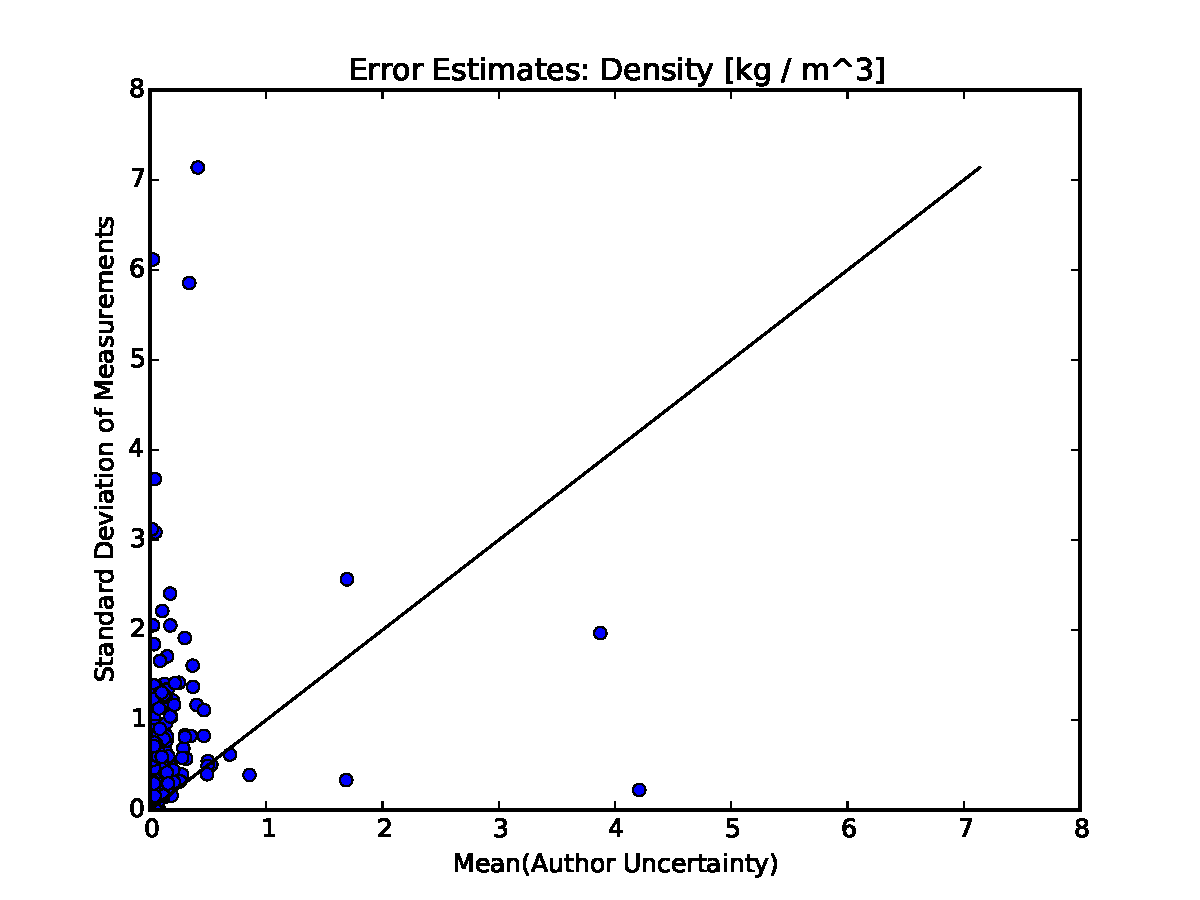
\includegraphics[width=8cm]{./figures/error_analysis_density.pdf}
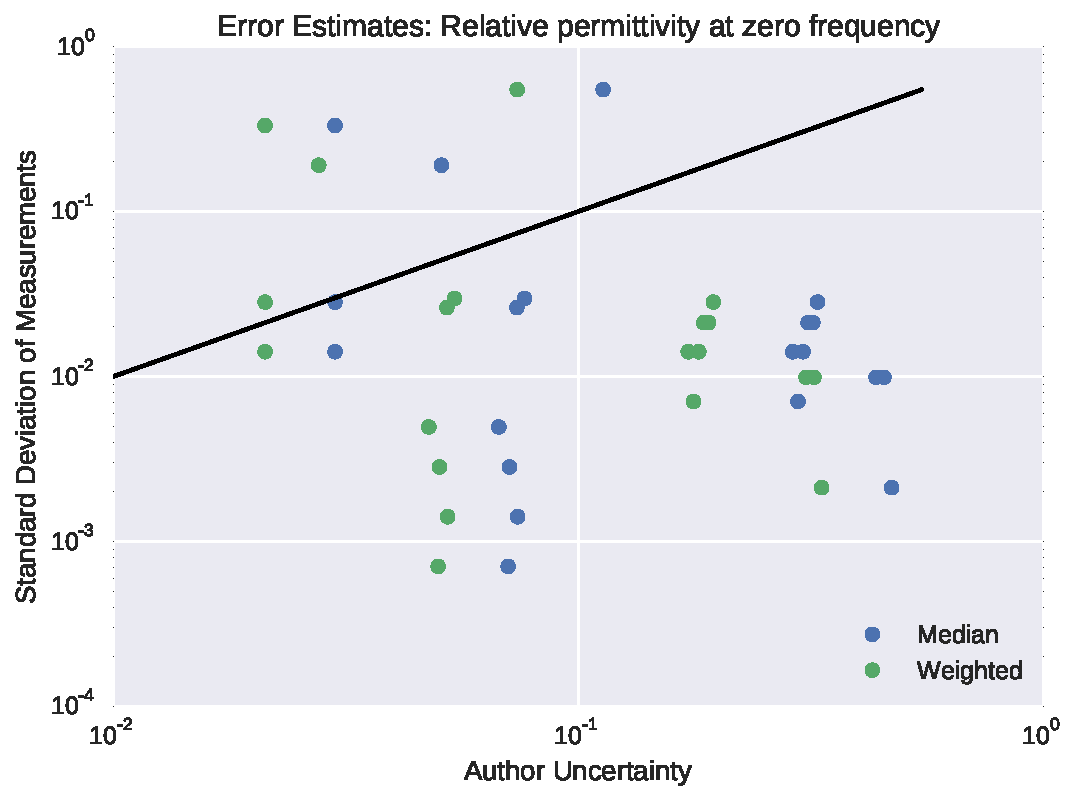
\includegraphics[width=8cm]{./figures/error_analysis_dielectric.pdf}

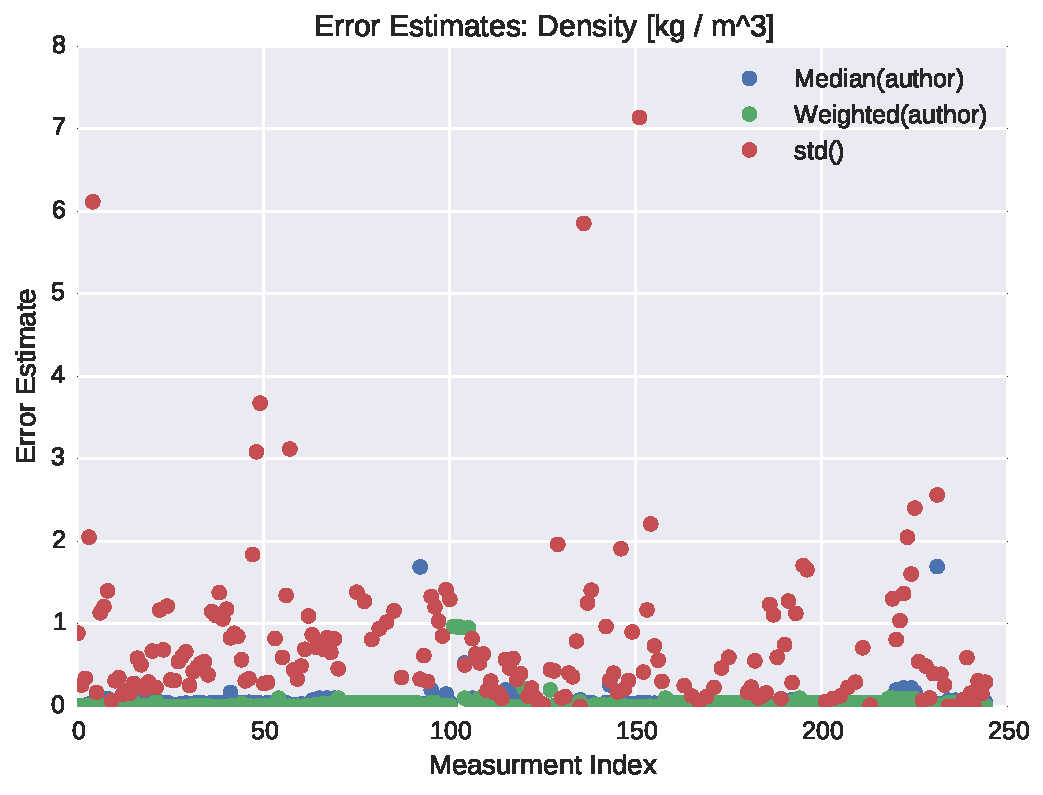
\includegraphics[width=8cm]{./figures/error_analysis_density_index.pdf}
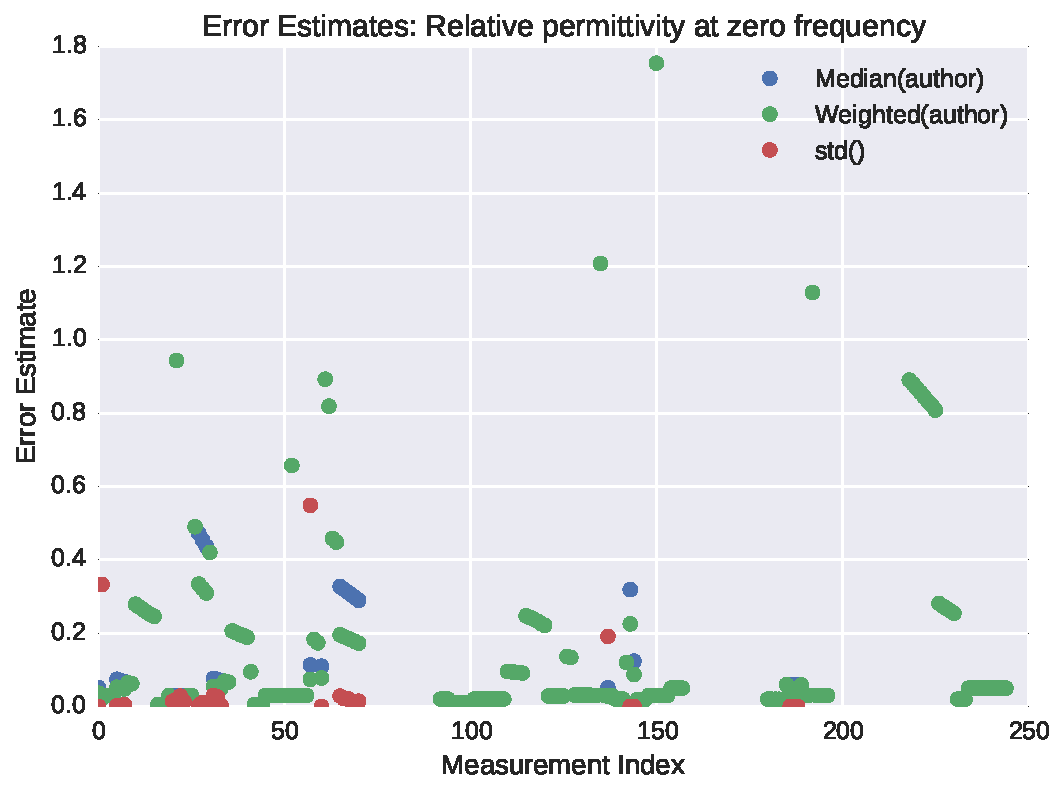
\includegraphics[width=8cm]{./figures/error_analysis_dielectric_index.pdf}

\caption{{\bf Assessment of experimental error in ThermoML data.}
To assess the experimental error in our benchmark set, we consider two orthogonal error measurements.  
The first is the mean of the uncertainties reported by the measurement authors.  
The second is the standard deviation of measurements in ThermoML.   
We see that author-reported uncertainties appear to be overly optimistic for densities (a, c), but author-reported uncertainties of dielectrics (b, d) appear consistent with the standard deviations.  
A simple psychological explanation might be that because density measurements are more routine, the authors simply report the accuracy limit of their hardware (e.g. 0.0001 g / mL for a Mettler Toledo DM40 \cite{mettlertoledo}).  
However, this hardware limit is not achieved due to inconsistencies in sample preparation; see Appendix in Ref.~\cite{chirico2013improvement}.  
Note that in panels (c, d) show the same information as (a, b) but as a function of the measurement index, rather than as a scatter plot---because not all measurements have author-supplied uncertainties, panels (c, d) contains slightly more data points than (a, b).  
}
\label{figure:ErrorAnalysis}

\end{figure}

%%%%%%%%%%%%%%%%%%%%%%%%%%%%%%%%%%%%%%%%%%%%%%%%%%%%%%%%%%%%%%%%%%%%%%%%%%%%%%%%
% FIGURE: DENSITIES VS TEMPERATURE
%%%%%%%%%%%%%%%%%%%%%%%%%%%%%%%%%%%%%%%%%%%%%%%%%%%%%%%%%%%%%%%%%%%%%%%%%%%%%%%%
\begin{figure*}

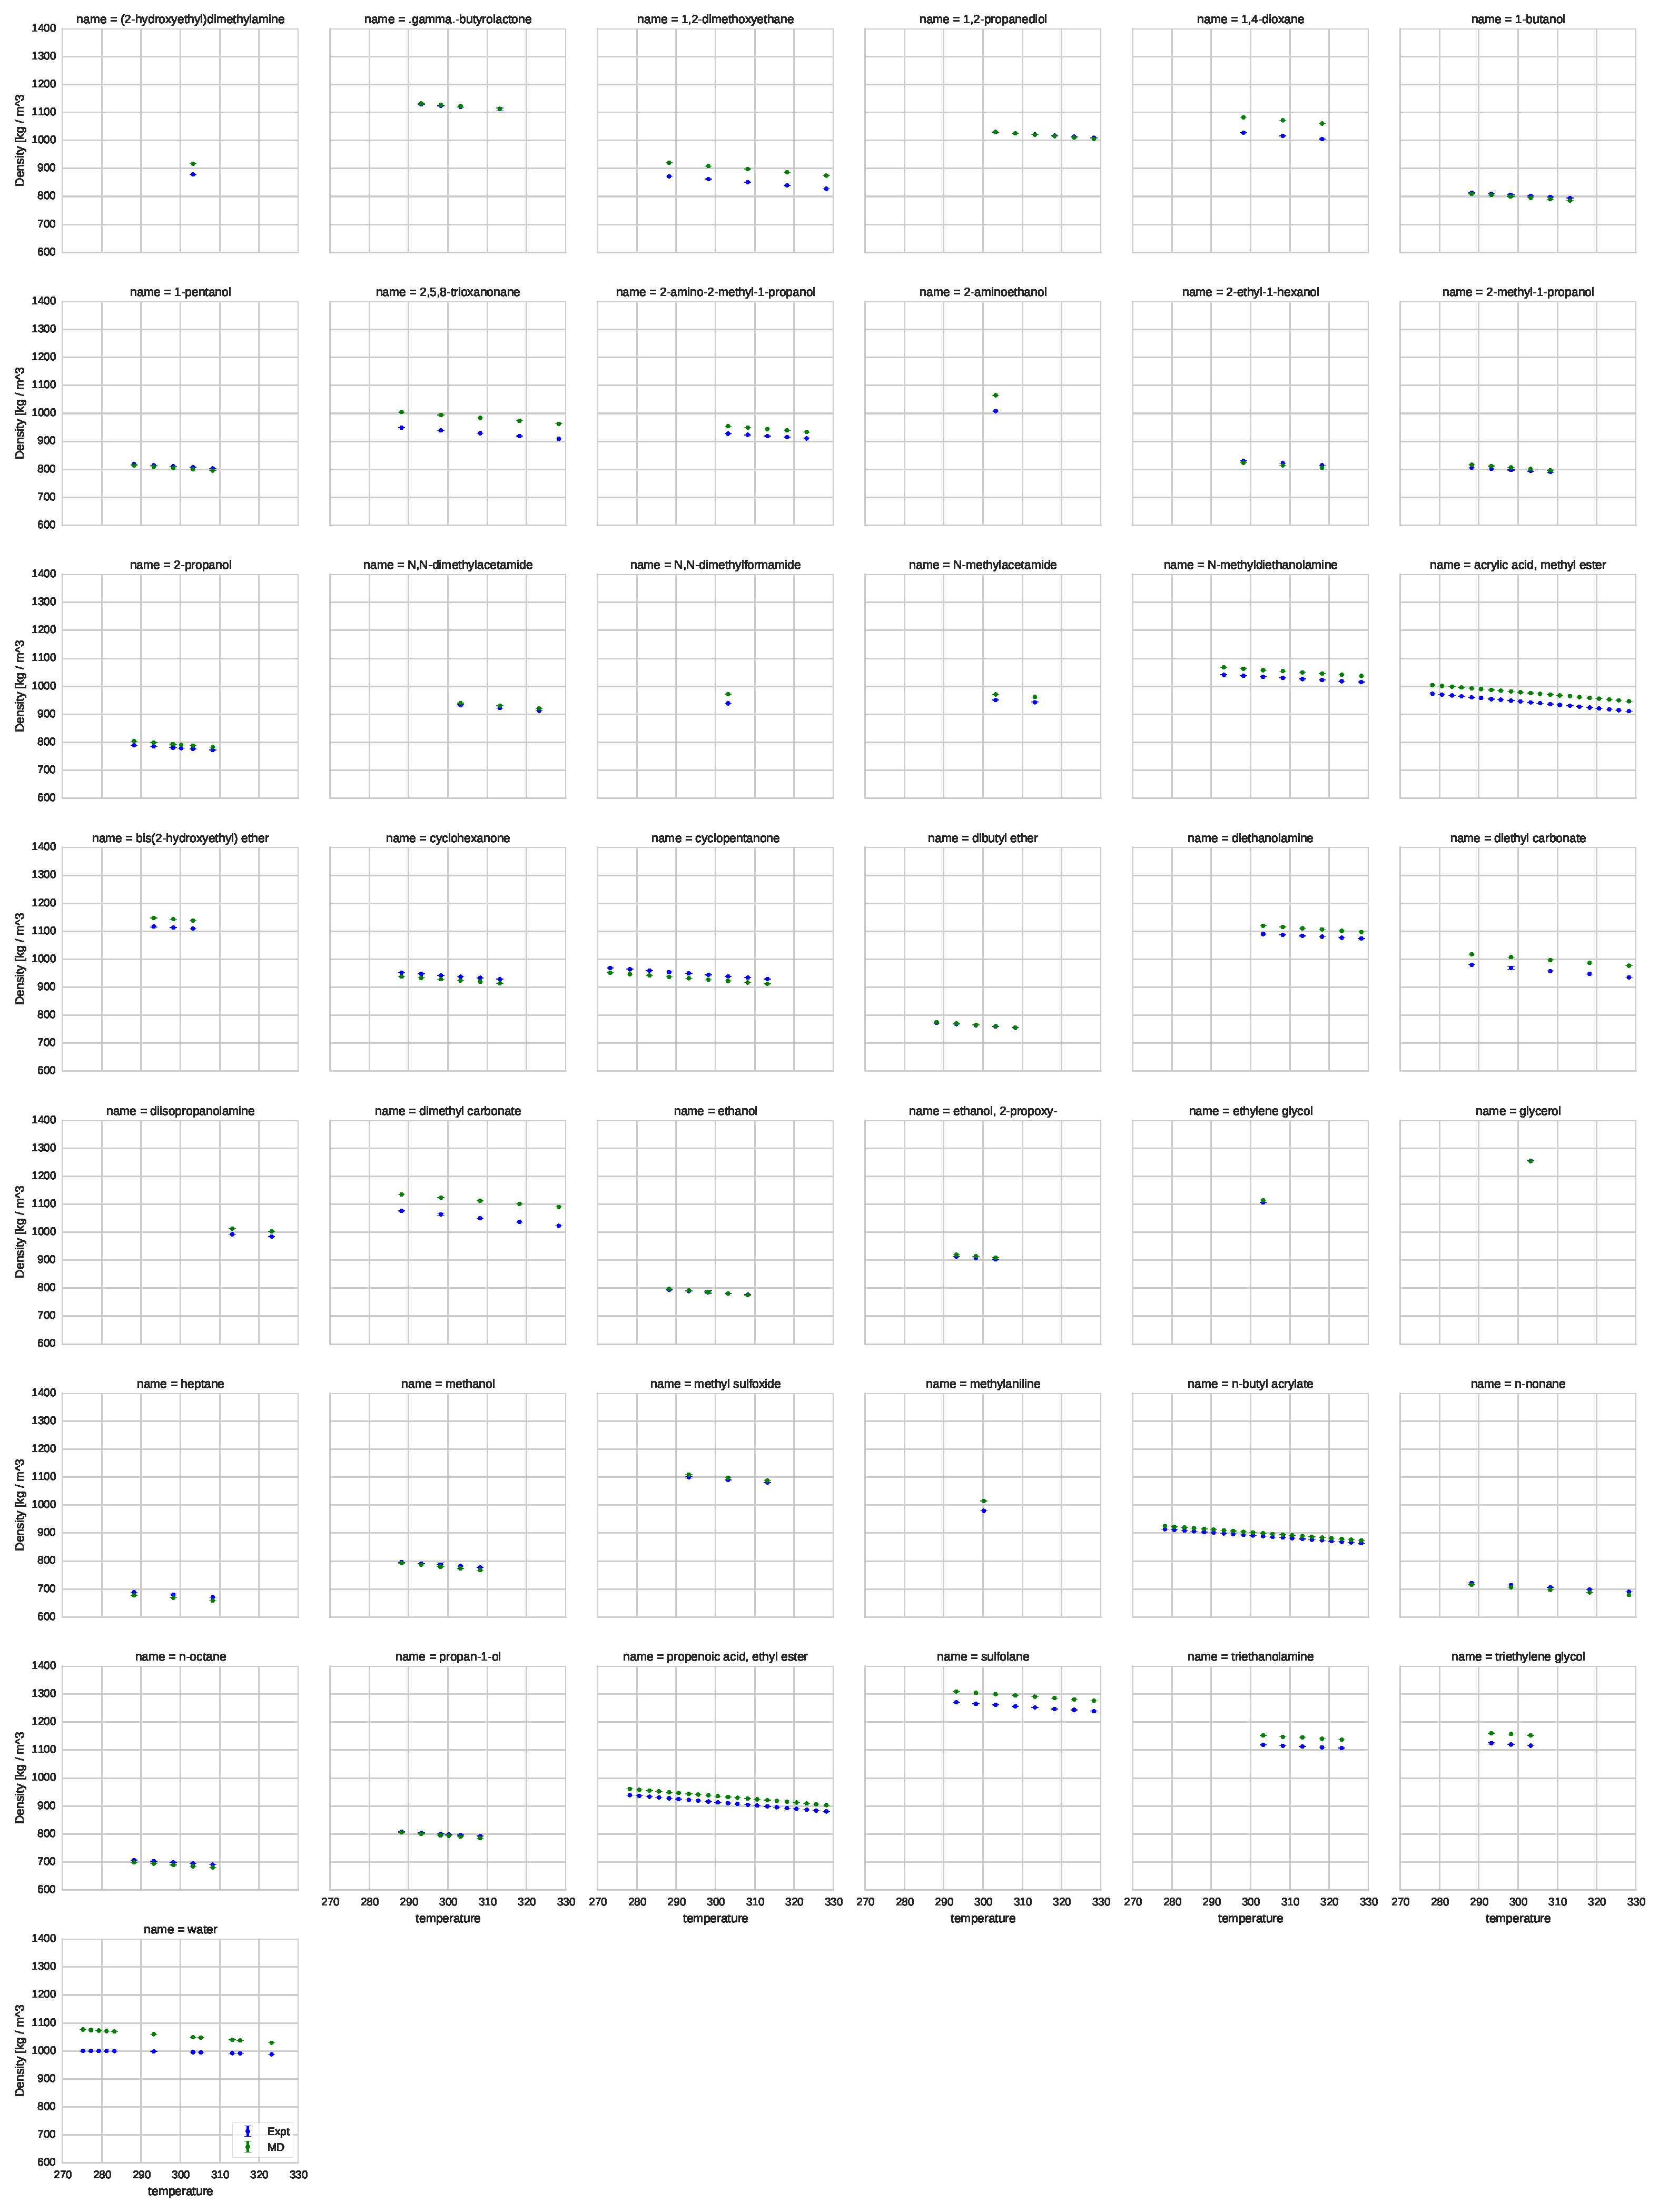
\includegraphics[width=\textwidth]{./figures/densities_versus_temperature_all.pdf}

\caption{{\bf Comparison of simulated and experimental densities for all compounds.} 
Measured (blue) and simulated (green) densities are shown in units of kg/m$^3$.
}
\label{figure:AllDensities}

\end{figure*}

%%%%%%%%%%%%%%%%%%%%%%%%%%%%%%%%%%%%%%%%%%%%%%%%%%%%%%%%%%%%%%%%%%%%%%%%%%%%%%%%
% FIGURE: DIELECTRIC VS TEMPERATURE
%%%%%%%%%%%%%%%%%%%%%%%%%%%%%%%%%%%%%%%%%%%%%%%%%%%%%%%%%%%%%%%%%%%%%%%%%%%%%%%%

\begin{figure*}

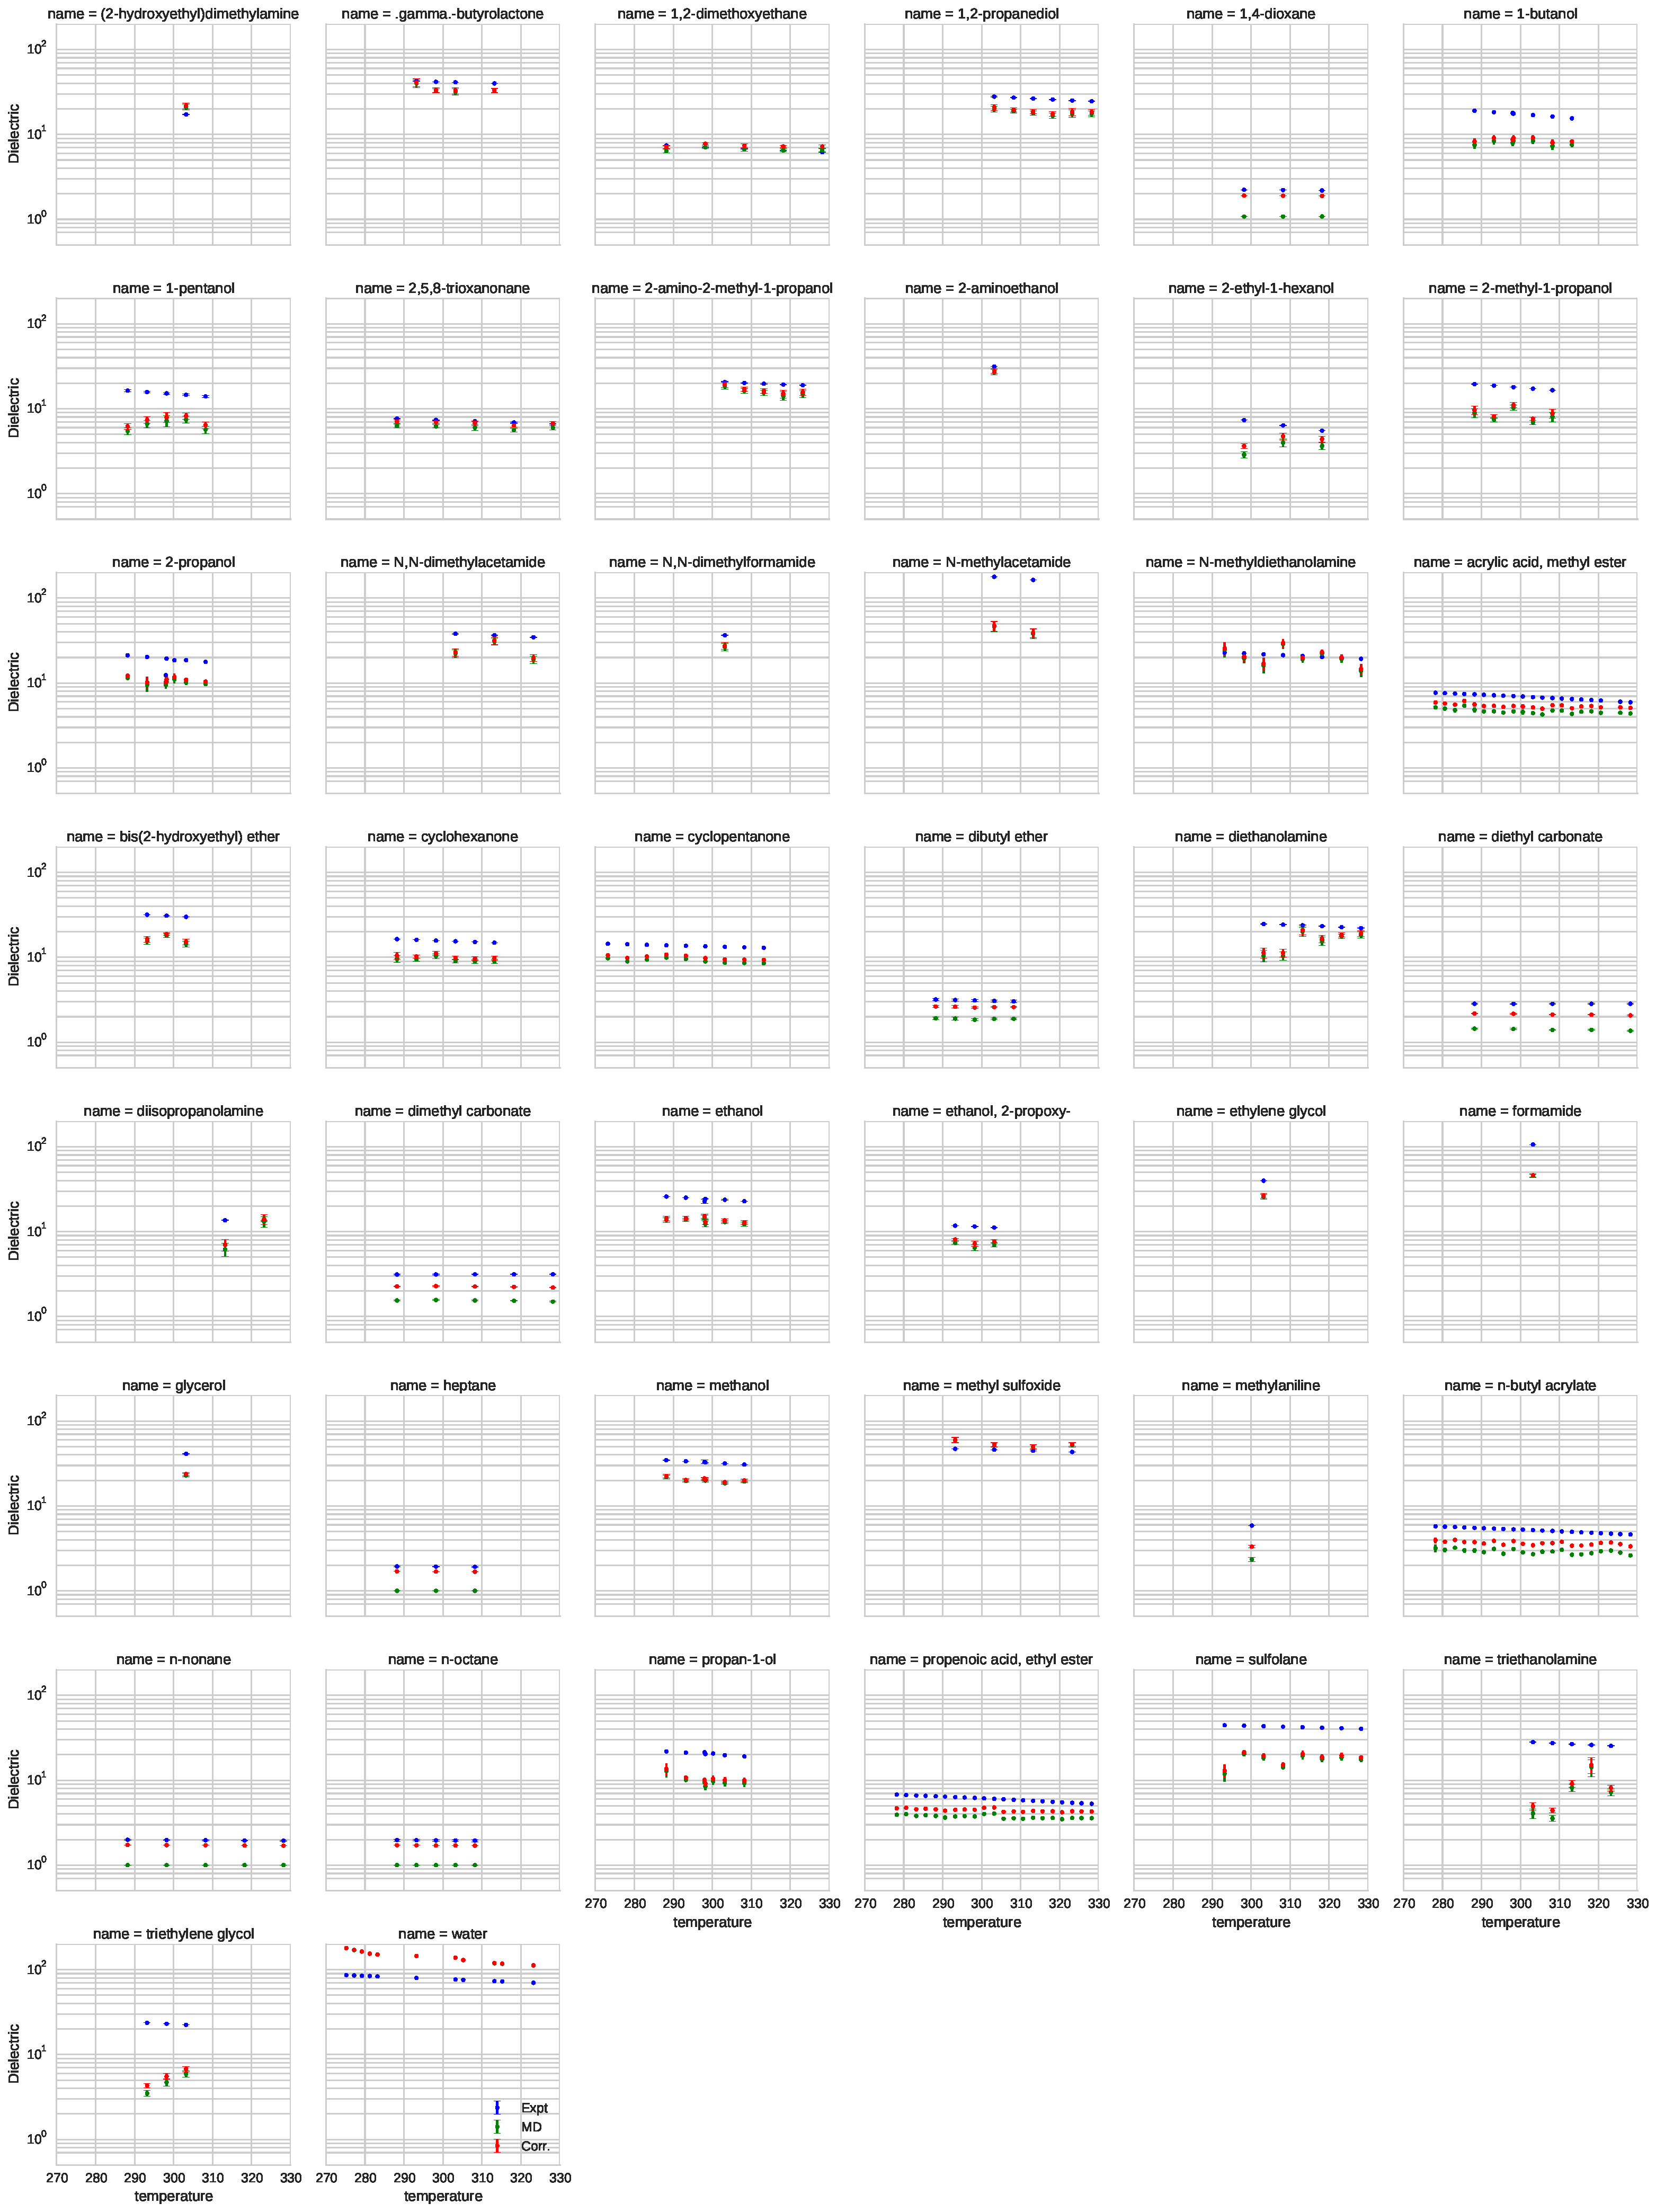
\includegraphics[width=\textwidth]{./figures/dielectric_versus_temperature_all.pdf}

\caption{{\bf Comparison of simulated and experimental static dielectric constants for all compounds.}
Measured (blue), simulated (green), and polarizability-corrected simulated (red) static dielectric constants are shown for all compounds.
Note that dielectric constants, rather than inverse dielectric constants, are plotted here.
}
\label{figure:AllDielectrics}

\end{figure*}

%%%%%%%%%%%%%%%%%%%%%%%%%%%%%%%%%%%%%%%%%%%%%%%%%%%%%%%%%%%%%%%%%%%%%%%%%%%%%%%%
% FIGURE: DIELECTRIC VIRTUAL CHEMISTRY
%%%%%%%%%%%%%%%%%%%%%%%%%%%%%%%%%%%%%%%%%%%%%%%%%%%%%%%%%%%%%%%%%%%%%%%%%%%%%%%%

\begin{figure}

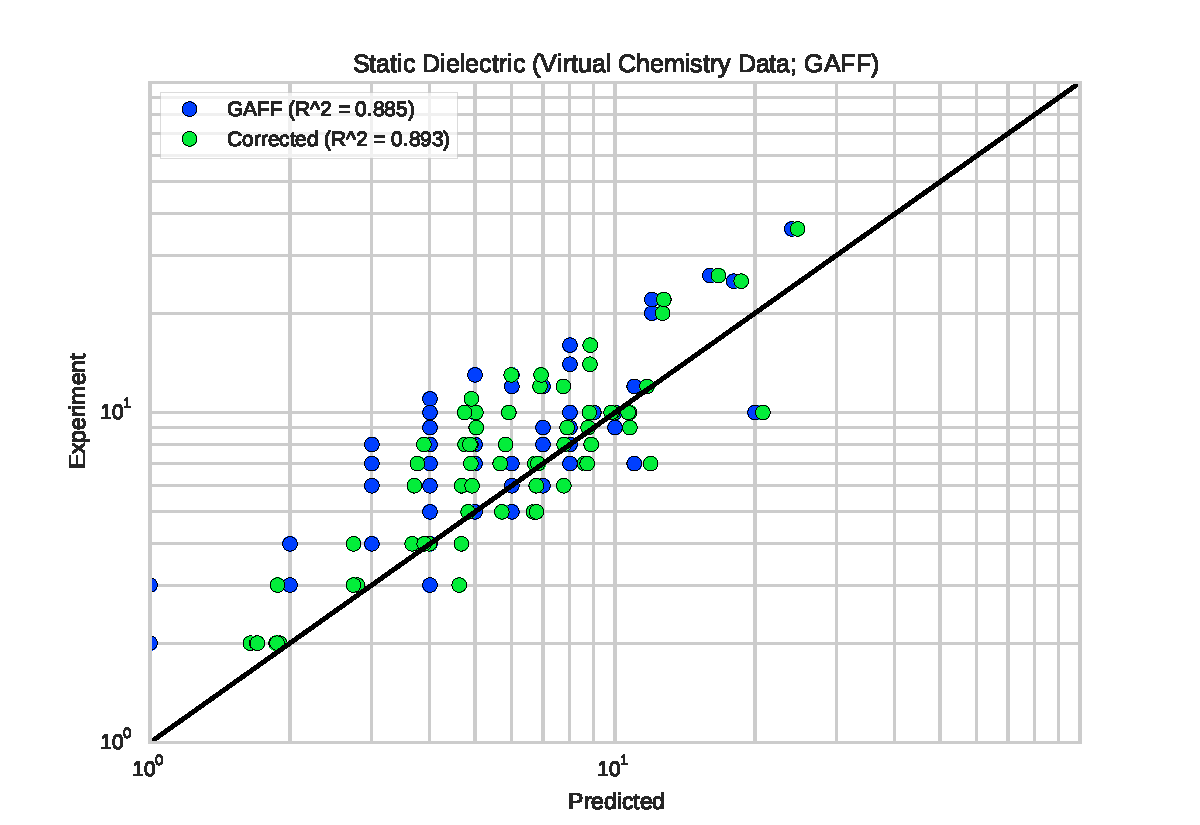
\includegraphics[width=\columnwidth]{./figures/dielectric_virtual_chemistry_gaff.pdf}

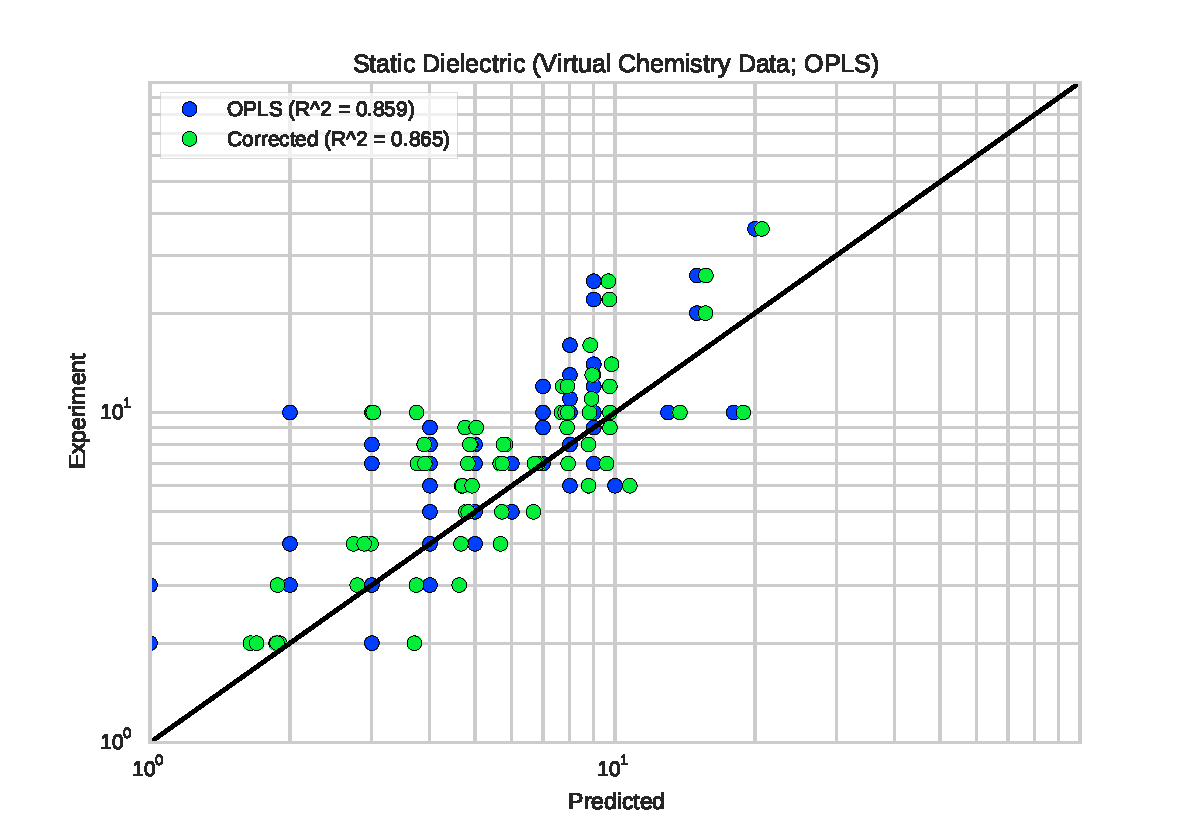
\includegraphics[width=\columnwidth]{./figures/dielectric_virtual_chemistry_opls.pdf}

\caption{{\bf Comparison of measured and simulated dielectric constants from the virtualchemistry dataset with and without polarizability correction.}  Measured (blue), MD (green), and MD + polarizability-corrected (red) dielectrics for the Virtual Chemistry dataset~\cite{caleman2011force, van2012gromacs}.  
}
\label{figure:VirtualChemistry}
\end{figure}


%\subsection{Dielectric Uncertainty}
%Following the discussion in \cite{horn2004}, we note that the static dielectric can be expressed as 

%$$\epsilon_0 = 1 + \frac{4\pi}{3k_B} \frac{\langle (M - \langle M\rangle)^2\rangle}{\langle V \rangle \langle T \rangle}$$

%We note that the dipole moment can be separated into vector components and expanded to give

%$$\epsilon_0 = 1 + \frac{4\pi}{3k_B} \frac{\langle M_x^2 \rangle + \langle M_y^2 \rangle + \langle M_z^2 \rangle - \langle M_x \rangle^2 - \langle M_y \rangle^2 - \langle M_z \rangle^2}{\langle V \rangle \langle T \rangle}$$

%We approximate the uncertainty using error propagation, e.g. $\delta(f)^2 \approx \sum_i (\frac{\partial f}{\partial x_i})^2 \delta(x_i)^2$

%$$\delta(\epsilon_0)^2 = \frac{4\pi}{3k_B}[(\frac{M}{T V^2})^2 \delta(V)^2 + (\frac{M}{T^2 V})^2 \delta(T)^2 + (\frac{1}{T V})^2 \delta(M)^2]$$

%$$ = \frac{4\pi}{3k_B}(\frac{M}{TV})^2[(\frac{\delta(V)^2}{V^2} + \frac{\delta(T)^2}{T^2} + \frac{\delta(M)^2}{M^2}]$$

%$$\delta(M)^2 = \delta(\langle M_x^2 \rangle)^2 + \delta(\langle M_y^2 \rangle)^2 + \delta(\langle M_z^2 \rangle)^2 + \delta(\langle M_x \rangle)^2 + \delta(\langle M_y \rangle)^2 + \delta(\langle M_z \rangle)^2 $$

\clearpage

\bibliography{benchmark}

\end{document}